\chapter{Overview}
\label{over}

%Little intro thing about science and stuff -- my story?

It is natural for humans to wonder how the world works.  % ``people''? ``how things work''?
Small children commonly ask a plethora of questions, 
sometimes pushing their parents to the point of exasperation.  
% quote on curiosity or someting?
I was one such child, always asking questions, and later %, 
devouring books and magazines, with a hunger to learn more.  
My first exposure to particle physics came at age eleven 
when I discovered my parents' copy of 
\textit{A Brief History of Time} by Stephen Hawking.  % REFERENCE
The ideas described therein -- fundamental particles 
with exotic properties, the flexible nature of spacetime, 
what might lie beyond the edges of our understanding -- 
boggled my mind, and I loved it.  
Over the following years I checked out much of the 
local library's collection of popular physics books.  
It is this desire to know more about the fundamental 
nature of the universe that has brought me to the point 
of pursuing a doctorate in experimental particle physics.  

%History
%short history of particle physics?
%quantum mech, cosmic ray detection with bubble chambers, etc, 
%first seeing the Z
%move on to accelerators
%talk a little about proton interactions, 

%maybe have all this history and the random definitions together 

\section{Short Overview of Particle Physics}
This hunger to figure out how things work has long 
been a part of human life.  
One of the most lasting questions has been 
``What, exactly, are things made of?'' 
%ancient greeks
The ancient Greeks tried to distill all matter into % DO I NEED TO REFERENCE ALL THE HISORICAL STUFF?  it came from wikipedia, and I would think it's common knowledge
four elements: fire, earth, water, and air.  % look up role of quintessence
They also came up with the idea of an ``atom,'' 
the smallest possible piece of matter, 
a piece that could be divided no further.  
%%galileo etc 
%In the Middle Ages, astronomers such as 
%Copernicus, Kepler, and Galileo 
%tried to formulate a system to 
%describe the motions of the heavenly bodies. 
%%enlightenment
%%newton
%Isaac Newton's laws of motion and gravitation %, 
%in the 17th and 18th centuries began the 
%``modern'' period of physics research.  
%They are still 
%recognized as valid in a wide physical context 
%and form the starting point for many 
%of today's introductory physics courses.  
%%1800's, maxwell
%Experimentation with electricity in the 18th and 
%19th centuries led to the first ``unification'' of forces: 
%James Maxwell's description of electricity and magnetism 
%in the same mathematical framework.   
%%early atom stuffs
%At this point research turned from phenomena 
%experienced in everyday life (magnets, gravity, motion) 
%to more esoteric effects.  
%% ADDED
%During the Middle Ages,
%Alchemists during the Middle Ages 
%recognized 
Natural philosophers through the ages 
discovered various chemical elements.  
However, not until relatively recently was 
the concept of the atom accepted scientifically. %, 
Up until the late 19th century, 
the issue was still debated.  
Dmitri Mendeleev's organization of the elements 
into a table according to the similarity of their properties 
hinted at an underlying structure.  
In addition, an atomic theory explained certain 
features of the behavior of gases, 
as applied by Ludwig Boltzmann and 
Amedeo Avogadro.  
However, the issue was not fully settled until 
the beginning of the 20th century.  
%This was when 
During this period 
Albert Einstein used an atomic theory of matter 
to explain the random motion of particles in a fluid %, 
(called Brownian motion after Robert Brown, who first observed it), 
and Jean Perrin verified the theory experimentally.  
Around this time progress was also being made 
on investigations into the structure of the atom.  
%% END ADDED
J.J. Thomson discovered that the cathode rays 
he was working with were 
made up of light, negatively-charged particles, 
dubbed electrons.  
He believed that these particles formed atoms, 
electrons floating in a sea of positive charge 
so that the overall element was electrically neutral: %.  
%This was 
the so-called ``plum pudding model.''  
However, experiments shooting positively-charged 
alpha particles at a sheet of gold foil demonstrated 
that the atom included a hard, positively-charged nucleus, 
illustrated in Figure~\ref{fig:AtomicModels}.  
This led Ernest Rutherford to propose the 
planetary model of the atom, in which the positive nucleus 
is orbited by a cloud of negative electrons.  
The model did not explain why the electrons did not 
lose energy and fall into the nucleus, though; 
this explanation came when Niels Bohr applied a 
quantized idea of energy to the atom.  
The quantum theory of light, 
proposed by Max Planck and Albert Einstein, 
said that light existed in packets of a given energy, 
known as quanta. 
%Essentially, 
Applied to the atom, it meant that 
electrons were only permitted to possess 
energy and angular momentum in discrete steps.  
They moved between these energy levels by absorbing 
or emitting light of specific energies.  
%Albert Einstein's special theory of relativity took on 
%motion at speeds approaching that of light, 
%while his later theory of general relativity 
%described gravity in terms of acceleration.  
%The scientific conception of the atom progressed from 
%a positive nucleus in a cloud of negative charge 
%to a nucleus being orbited by electrons 
%in a set of specific energy states.  
%more detailed modern stuff: 40's, 50's, etc -- quarks, strange, muon, W and Z. 
Rutherford later noticed that the atomic masses 
were roughly integer multiples of the hydrogen mass; 
he proposed that atomic nuclei were made of 
positively-charged protons, 
and later added electrically neutral neutrons 
to make up the needed leftover mass.  
Meanwhile, quantum mechanics was soon formulated to describe 
the properties of particles' behavior in terms of waves 
of quantized energy.  
%The study of these fundamental particles took off 
%%during this time period, 
%after this, 
%with the proposal of a relativistic quantum theory %, 
%and the discovery of antimatter and the muon.  
Paul Dirac formulated a quantum theory that was consistent 
with Einstein's special relativity, 
which dealt with motion at speeds approaching that of light.  
In addition, the idea of forces being mediated by the exchange 
of force particles was gaining traction: 
quantum electrodynamics formulated the electromagnetic force 
as the interaction between charged particles and photons, 
or particles of light.  
%The force holding protons and neutrons together in the atomic 
%nucleus was posited to be mediated by another particle, 
%called the pion.  
At this point many new particles were being discovered, 
including the pion, 
such 
%as well 
as the positron and the muon, 
along with a large number of heavier particles.  
Quarks were proposed in Murray Gell-Mann's Eightfold Way 
to explain the many new heavy particles 
being found. % 
The quark model successfully explained the 
properties of neutrons and protons: 
those particles along with some of the new discoveries 
were ``baryons,'' made up of three quarks, 
while other new particles were ``mesons,'' 
made up of a quark and an anti-quark.  
The force between the quarks was the same one 
keeping the protons and neutrons together inside the 
atomic nucleus, 
mediated by particles called gluons.  
Since it was strong enough to overcome the repulsion 
between the positively-charged protons, 
it was called the strong force.  
%and were later verified experimentally.  
%The decay of the neutron and the observation of neutrinos 
%interacting with electrons necessitated 
Another force, called the weak force, 
was known to be responsible for the decay of 
neutrons into protons.  
Through the development of modern particle theory, 
it was predicted that heavy particles mediated this force.  
The discoveries of these particles, the W and the Z bosons, 
marked a success for the current theory: 
it had predicted particles that had previously been 
undiscovered.  

 \begin{figure}[htb]
  \begin{center}
    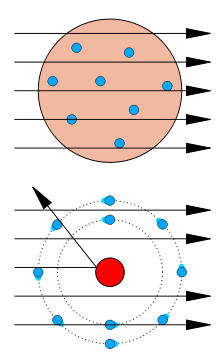
\includegraphics[width=240pt]{Figures/overview-220px-Gold_foil_experiment_conclusions_svg.png}
  \end{center}
  \caption[The ``plum-pudding'' and the planetary atomic models. ]
	  {The ``plum-pudding'' and the planetary atomic models. 
	    Observations showed incident particles back-scattering 
	    consistent with the dense, positive nucleus of 
	    the planetary model. 
	  }
  \label{fig:AtomicModels}
 \end{figure}



%recent accelerators: top. higgs and beyond...
Experiments making all these particle discoveries 
have progressed from observing cosmic rays 
in cloud chambers and bubble chambers 
to observing collisions created in higher- and higher-energy 
accelerators 
(hence the current name of the field, 
``high-energy physics'').  
Most recently, the last of the six quarks, the top quark, 
was discovered at the Tevatron accelerator in 1995.  
All these particles and their interactions are described 
within the framework of the Standard Model of particle physics; 
the Standard Model combines the quantum electrodynamics 
of charged particles and photons, the quark and gluon model, 
called quantum chromodynamics, 
and the interactions of the weak force into one framework.  
%(The Standard Model, including the full set of particles 
%and their interactions, will be more fully 
%developed in Ch.~\ref{theory}.) 
The Standard Model will be further explained in 
in Chapter~\ref{theory}. 
Currently, the Standard Model is considered to be the 
primary description of particle physics.  
However, it predicts one particle that has not yet been 
observed, the Higgs boson.  
Finding the Higgs and verifying this last piece 
of the Standard Model 
is one of the current goals of 
particle physics.  
However, there are observations that 
the Standard Model cannot explain, 
such as the fact that neutrinos have mass.  
The Standard Model is also incomplete in that 
it does not incorporate the last fundamental force, gravity.  
Further, some physicists think that various additions 
to the Standard Model make it more elegant.  
These new models predict various new particles.  
Therefore, scientists are also on the lookout 
for any evidence of particle physics existing 
outside the Standard Model.  
%One particle predicted by the Standard Model has not yet 
%been discovered, the Higgs boson; 

%   * particles?  although that's theory intro (but need SOME particle-specific stuff) 
%ref ch 2 -- or wherever end up putting standard model section, maybe move to ch 1!
%some kind of short little intro, motivate need to define those following terms,
%want to talk about Z and why important, motivations


%   * ``high-energy''
%``High-energy'' physics refers to modern particle physics. 
%In the beginnings of particle physics, 
%the available accelerators operated at much lower energies.  
%Low-energy accelerators are still used in nuclear physics 
%and aid in materials physics and biophysics studies. 
%However, to probe the fundamental interactions between particles, 
%today's accelerators use much higher energies.  

%TACK THE DEFINITIONS ONTO THE END OF WHATEVER THE PREVIOUS 
%(INTRODUCTORY) PARAGRAPH WAS

%Z boson and history, decay and detecting electrons, history of electrons?
%Z important to LHC


\section{Introduction to the Z Boson}
% Z background
This analysis studies the production of the Z boson.  
The Z is one of the particles that mediates the weak force.  
It was first observed in 1973 in the Gargamelle bubble chamber at CERN 
when an electron would sometimes apparently start moving on its own 
\cite{NC-Gargamelle}.  
This was understood to be due to a neutrino striking the electron 
(by their nature, neutrinos rarely interact with matter and so are generally 
not seen in particle detectors).  
However, it was not previously known that neutrinos could interact 
with electrons in this way.  
This new interaction implied the existence of a new particle, the Z, 
as had been predicted by electroweak theory.  
The Z was not observed directly until a decade later, 
when it was produced in proton collisions in the 
Super Proton Synchrotron (SPS) accelerator at CERN in 1983 
\cite{Z-ua1}, \cite{Z-ua2}.  

% Z properties
The Z has a relatively large mass, 
like the other mediator of the weak force, the W; 
however, unlike the electrically-charged W, the Z is chargeless.  
The Z interacts with all matter particles (as opposed to force carriers); 
it can be formed in a high-energy interaction between 
two particles that are oppositely-charged but otherwise alike.  
This includes the quark constituents of protons, 
which means it can be formed in the proton-proton collisions 
of the LHC.  
The Z can also decay into similar pairs of particles, 
one such possible pair being the electron and the positron; 
this is the decay studied in this analysis.  

% Z motivation
The Z has been well-studied in previous experiments, 
which makes it an ideal initial study for the LHC experiments 
\cite{PhysicsTdr}.  
Its mass is well-known enough to be used to 
adjust the experiments' energy scales.  
In addition, the fact that the Z is produced from the 
constituents of protons 
means that it can shed light on the protons' internal structure.   
The Z also tends to decay in a similar way as the 
proposed Higgs boson. %, 
%which is the only particle in the Standard Model that 
%has yet to be observed.  
A particular Z decay signature may 
look like the Higgs and vice versa.  
Therefore, in order to look for the Higgs, 
the decays that look like it must be very well-studied.  
This way, if the Higgs is seen, 
it will be known that it is definitely something new.  


%\section{Terms in particle physics, technical stuff}
\section{Useful Concepts}

%the practical purpose of MC -- can simulate all stages of gen/sim/reco/etc and compare 
%everything step-by-step with data, as well as of course getting some quantities 
%that require extra knowledge, like acceptance (and predicting efficiencies, rates, etc)
%HA, that sounds like a few of those things in the pythia manual intro!  and I came 
%up with them myself!  

%glossary? (explanatory text, with true glossary in appendix?)  

%Introductory terminology?  put terminology section in beginning?

A few definitions and concepts should be introduced 
before moving on to more specific explanations 
of the analysis.  
%   * ``kinematic'' 
In the following pages, much will be described by the word 
``kinematic'' or ``kinematics''.  
This refers to the properties of position or motion.  
So, ``kinematic criteria'' means selections applied according to 
quantities such as momentum or angle.  
Often, a calculation may need to deal with 
the full range of possible values 
for multiple quantities, 
%may need to be dealt with, 
or the ``phase space.'' 
%   * statistical and systematic uncertainties or errors
%   * ``phase space''! 
Phase space refers to the collection of total 
possible values for a set of quantities.  
A given system is represented by one set of 
values out of that collection.  
%Direction (in three dimensions)   % NOT ACTUALLY TRUE!!!
%plus speed or energy define a 
%four-dimensional phase space 
%for a particle's kinematic quantities.  
For some calculations it is necessary to include 
contributions from the entire phase space, 
for example integrating over all possible 
angles for a particle's direction.  

%   * events
Experimental particle physics is built on ``events.''
An event is the name for is a particle interaction, 
particularly one 
that has been captured and recorded by the detector.  
%   * signal, background.  
In general, %events that contribute to the specific process     
events caused by the specific process     
being studied are termed ``signal,'' 
while any events 
%that do not contribute 
from other sources 
are called ``background.'' 
A significant part of any analysis is designing 
criteria that select signal events while 
rejecting background events, 
so that the analysis focuses only on data containing 
that process.  
The number of events for a given signal can be used 
to calculate quantities of interest, 
for example how often that process  
occurs relative to others.  

\section{Anatomy of an Event}
%Like, what actually happens!

%this section sets the context and introduces 
%terminology

A proton-proton interaction begins 
with beams of protons accelerated 
in opposite directions.  
The protons are formed into ``bunches,'' 
with many, many millions of protons per bunch.  
These beams of proton bunches are directed to 
cross at the center of the detector.  
%Most such ``bunch crossings'' do not result 
%in a significant interaction.  % interaction at all? YES, DUH pileup
In an encounter between two protons, 
the fundamental interaction takes place 
between individual ``partons,'' 
which is the collective term for 
the quarks and gluons that make up the proton.  
Each ``bunch crossing'' results in 
a small number of interactions, 
the majority of which do not interact 
strongly enough to be interesting.  
However, sometimes two partons %, 
%i.e. a quark or gluon inside the proton, 
%interacts very strongly with a parton 
%from another proton.  
from separate protons interact very strongly.  
These are the types of interactions 
that are typically interesting.  
%   * ``hard'' vs ``soft''
%A ``hard'' interaction is one in which the partons 
%interact very energetically.  
An interaction in which the partons interact 
very energetically is a ``hard interaction.''  
Conceptually, the partons ``hit each other hard.''  
Hard interactions are typically detected 
by having end-product particles with 
a lot of momentum 
in the transverse direction, 
perpendicular to the protons' original 
direction of motion.  
Only in hard interactions is the original 
momentum disturbed so much; 
in ``soft,'' or low-energy, interactions, 
most of the protons' momentum 
continues in the same direction, 
down the beam-pipe.  

Oftentimes the two partons exchange 
a particle, such as a photon or gluon.  
In other cases another particle is produced, %formed, 
such as a Z boson; 
this is the scenario 
studied in this analysis.  
Particles formed in this way 
are typically heavy and therefore 
short-lived, 
decaying into lighter, more stable particles.  
This analysis studies the Z's decay into two 
electrons, 
which are the lightest charged particles 
and therefore (to conserve charge) 
do not decay.  
These decay products are what fly ``out'' 
into the detector with 
some energy and direction, 
and it is these quantities 
that are measured by the detector.  

However, additional processes may contribute 
to the signature left in the detector.  
One of the initial partons 
or final decay products 
may radiate an additional particle 
which then ends up in the detector.  
This is known as ``initial-state radiation'' (ISR) 
and ``final-state radiation'' (FSR) respectively.  
In addition, there are two ways that 
particles unrelated to the hard interaction 
may show up in the detector: 
underlying event and pileup.  
The ``underlying event'' refers to the 
interactions taking place between the 
proton remnants, 
the parts of the proton ``left over'' 
from the hard interaction.  
``Pileup'' refers to any interactions that happen 
between other protons in the bunch.  
%These are generally soft, 
%low-energy interactions.  
Statistically, at most only one hard interaction 
happens in any given bunch crossing; the rest are soft.  
Both underlying event and pileup can contribute 
energy deposits that are recorded as part of the event.  
Typically they are both fairly low-energy and 
therefore easily filtered out as background.  

%hits, reconstruction, triggering?  
%selection out of reconstructed objects

Fully-decayed, end-product 
particles leave a signature in the detector 
by interacting with its material.  
Some detector material emits light when 
particles pass through; 
in these materials, the amount of light 
is proportional to the energy of the particle.  
Other parts of the detector rely on an 
electric signal generated 
as the particle passes by.  
%A series of these signals, close together in space, 
%can be linked together
These particle interactions with the detector 
are collectively known as ``hits.''  
In the process of reconstruction, 
hits are linked together to 
follow the path of the particle that caused them.  
For example, a series of hits in the tracker 
could show the trajectory of a charged particle 
as it passed through.  
The curvature of the trajectory could be measured 
and turned into a value for the momentum, 
knowing the value of the magnetic field.  
This track could then be linked 
with a significant emission of light 
in the calorimeter.  
If the energy from the light 
matches the momentum from the track, 
this object is reconstructed as an electron.  
A rough, on-the-fly reconstruction 
process takes place in real time to decide 
whether or not to save the event, 
%which is 
called triggering.  
Saved events undergo a more thorough 
reconstruction of their detector signals later, 
since this more thorough version 
takes too long to do in real time.  
However, not all objects reconstructed as 
a given particle are actually due to 
a real particle of that type 
passing through the detector.  
Some reconstructed objects are ``fakes.''  
These fakes are typically selected out 
by more stringent criteria on various 
particle properties. %, 
However, this selection is done at the analysis level, 
not during reconstruction.  

\section{Measurement of Cross Section}
\label{over:xsec}

%   * cross section!
The cross section, the quantity being calculated in this analysis, 
%is such a measure of ``how often things happen.''  % REWORD TO HAVE IT NOT RIGHT AFTER ``EVENT''
is a measure of ``how often things happen.''  
However, it is not measured as a rate (occurrences per unit time); 
instead it is measured as a cross-sectional area 
and represents the probability of the given interaction occurring.  
An analogy may be made to trying to hit a target with a tennis ball.  
The bigger the target is, the more likely you will be able to hit it.  
The sizes of both objects matter: 
a trajectory that would cause a tennis ball to just miss the target 
would cause a basketball to clip the edge, 
solely because of the basketball's larger size.  
Therefore ``cross section'' may be more precisely defined as the 
effective cross-sectional area of the target, 
taking into account the sizes of both the target and the projectile.  
When both the target and projectile are particles, %such as protons, 
they may interact ``at a distance,'' that is, without ``touching'' each other, 
through the fundamental forces.  
(For example, electrons are thought to be point particles 
and therefore have no spatial extent, 
but they still attract and repel other particles 
through the electromagnetic force.) 
This interaction-at-a-distance increases the effective cross section.  
An interaction involving two particles that 
interact with each other very strongly has a large cross section.  
The cross section depends on the strength of the force between them.  
%FORMULA AND EXPLANATION HERE??

According to the definition, ``interaction cross section'' applies only to 
the particles doing the colliding.  
However, a cross section is usually associated with the entire process, 
such as (in this case) 
$ q\bar{q} \rightarrow Z/ \gamma^{*} \rightarrow e^{+} e^{-} $.  %include ggF?? or other methods of Z prod?? put all relevant feynman diagrams in theory section...
Here, the number calculated as the cross section takes into account 
only those events where a \Zg is formed, 
as well as the fact that only some of those events decay into electrons.  
The fraction of events that decay to a certain final state is known as 
the branching ratio, abbreviated BR.  
When it is not explicitly mentioned along with the cross section 
for a given final state, it is understood to be included.  
Adding up the cross sections for all of these possible interactions 
would give the full proton-proton interaction cross section.  

The cross section $\sigma$ is related to the event count $n$ by 
\[
n = \sigma \times \mathcal{ L }
\]
$\mathcal{ L }$ in this equation is the ``luminosity,'' 
a measure of the number of proton collisions.  
Two types of luminosity are spoken of in particle physics: 
instantaneous luminosity and integrated luminosity.  
Instantaneous luminosity, denoted here by $L$, 
refers to the rate of potential proton interactions.  
Specifically, it is defined as the number of protons 
passing through a given area in a given amount of time.  
(The units are therefore 
$\frac{1}{\mathrm{area} \times \mathrm{time}}$, 
typically cm$^{-2}$s$^{-1}$.)  
If the same number of protons are squeezed into a smaller area, 
the instantaneous luminosity is higher; 
the protons in the colliding beams are more likely to interact.  
This is analogous to trying to walk through a room with many 
other people in it; 
you are much more likely to bump into people in a small, crowded room 
than a large room in which the people are much more spread out.  
% is luminosity measured per beam or what??
% how is it measured otherwise??
% how much the beams overlap affect it...
Integrated luminosity, or $\mathcal{ L }$ here, 
is the instantaneous luminosity accumulated 
over a definite period of time, 
effectively the total number of protons 
that have passed through a unit of area.  
(Integrated luminosity is measure in units of 
$\frac{1}{\mathrm{area}}$, the conventional unit 
being powers of the \textit{barn}, 
equal to $10^{-28}\mathrm{m}^2$.)
It is a measure of the total amount of data gathered.  
The luminosity in the above equation refers to 
the integrated luminosity.  
Essentially, the equation says that 
the total amount of data (the luminosity) 
times the likelihood a specific interaction will happen 
(the cross section) 
gives you the total number of events of that type 
that have happened (the event count, $n$).  
In practice this formula must be modified 
to account for the natural limitations of the detector: 
Two new factors, $A$ and $\epsilon$, must be introduced.  
$A$, the ``acceptance,'' accounts for the fact 
that the detector cannot be designed in a way 
that allows it to see every possible particle.  
In particular, any particles that continue 
in the direction of the proton beam will be lost -- 
the presence of the beam pipe precludes 
detector material in that direction.  
%In addition, due to the large magnetic field 
%used within the detector, 
%a particle with a low enough energy may 
%spiral around inside, not actually hitting 
%the calorimeter.  
The value of the acceptance is the fraction 
of the events that can theoretically 
be seen by the detector, %.  
often defined in terms of %as %to be within 
a region of kinematic phase space: % PUT KINEMATIC AND PHASE SPACE DEFS BEFORE THIS
``above energy X and within angular constraints Y.''
For simplicity's sake, 
these constraints are typically chosen to include 
only regions of the detector 
and particle energies 
for which the particles of interest can be well-reconstructed.  
The ``efficiency,'' $\epsilon$, 
takes into account the fact that 
even for particles that leave a definite 
signature in the detector, 
they may still not be recorded as such.  
High efficiency is a primary goal of any 
experiment, 
but the sources of inefficiency can never be 
completely eliminated.  
The efficiency is often broken down into 
efficiencies of the individual steps: 
\[
\epsilon = \epsilon_{ trig } \times \epsilon_{ reco } \times \epsilon_{ sel }
\]
The individual efficiencies correspond to 
triggering, reconstruction, and selection.  % DEFINE THESE BEFOREHAND
The boundary between what is considered 
for the acceptance versus for the efficiency 
is somewhat fluid: 
failing to record a particle 
with a very low energy may be 
considered an issue of acceptance 
%defined as being outside the acceptance 
(because the detector is not designed 
for such small energies) 
or a matter of efficiency 
(because though the particle left 
a signature in the detector, 
it was not reconstructed).  
It is merely a matter of definition, 
and in the end result makes no difference.  

The inclusion of acceptance and efficiency 
turn the previous expression 
of event count and cross section into 
\[
n = \sigma \times \mathcal{ L } \times \epsilon \times A
\]
The number of events actually seen ($n$) is reduced 
by the factors accounting for the detector limitations.  
In order to calculate the cross section $\sigma$ 
(including the branching ratio) 
of the 
$ q\bar{q} \rightarrow Z/ \gamma^{*} \rightarrow e^{+} e^{-} $ 
interaction, 
which is the quantity this analysis aims to get, 
the equation must be rearranged into 
\[
%\sigma_{ Z } \times \textrm{ BR }_{ Zee } = \frac{ n_{ Zee } }{ \mathcal{ L } \times \epsilon \times A}
\sigma_{ Z } \times \textrm{ BR }( Z \rightarrow ee ) = \frac{ n_{ Z \rightarrow ee } }{ \mathcal{ L } \times \epsilon \times A}
\]
Now $\sigma \times \textrm{ BR }$ is expressed 
in terms of other quantities which 
can be measured or calculated.  
This equation is the heart of this analysis.  
The ``meat'' of the analysis is then 
measuring the quantities that combine to 
make up the cross section, 
and putting it all together.  


\section{Reference Frame and Coordinates}

%   * center of momentum reference frame

For some high-energy physics experiments, 
there is a choice of several reference 
frames that can be used for measurement, 
each with their own benefits.  
However, in the case of proton-proton collisions, 
the logical reference frame for measurements is 
the frame at rest with respect to the detector, 
the ``lab frame,'' 
because it is the same as the 
proton-proton center of momentum frame.  
Therefore all measurements are done 
in the lab frame.  
%If the two particles have the same energy but opposite 
%direction, according to some observer, 
% then this observer is in the system's 
%center-of-momentum frame.  


%   * eta/y, phi

A particular set of coordinates is often used to describe 
the direction of outgoing or intermediate particles.  
The direction of the incoming particles defines an axis, 
the beam axis.  
The azimuthal angle, measured around this axis 
and analogous to longitude on the earth's surface, 
is labeled $\phi$.  
The angle along the axis, the polar angle 
(analogous to latitude), 
is labeled by $\theta$.  
However, it is much more common to measure this 
angle in terms of pseudorapidity, $\eta$, 
which is given as a function of $\theta$:
\[
\eta = -\ln \left[ \tan \left( \frac{\theta}{2}\right) \right]
\]
$\eta$ is preferred because of its relation to another quantity, 
rapidity, $y$, which is a function of the particle's 
energy and momentum:
\[
y = \frac{1}{2} \ln \left( \frac{E+p_L}{E-p_L} \right)
\]
where $p_L$ is the longitudinal component of the 
particle's momentum (the component parallel to the beam axis).  
% WON'T DO COMPOSITION OF VECTORS
Rapidity is useful when dealing with relativistic speeds, 
such as those at which the particles typically travel.  
When viewed from separate reference frames that are moving 
at relativistic speeds with respect to each other, 
a particle's speed, direction, and energy appear to be different.  
However, rapidity has special status in that the 
difference in rapidity 
between two particles does not change 
when the reference frame is changed.  
A particle's rapidity can be approximated by the 
pseudorapidity if it is very light or 
traveling very fast 
(pseudorapidity is identical to rapidity 
if the particle has zero mass, 
in which case it is also 
moving at the speed of light).  
In addition, outgoing particles tend to be 
distributed uniformly in terms of rapidity, 
as opposed to the polar angle $\theta$, 
which does not enjoy the same uniform distribution. 
Since rapidity itself is not a measure of angle, 
pseudorapidity is used as the coordinate.  
Rapidity is calculated in cases 
where the particle of interest may be heavy 
and may not have a high speed, 
for example the Z boson examined in this analysis.  

%\section{General Analysis Software}
\section{General Analysis Tools} % changed from ``considerations''

% RANDOMMMMMMM

A few concepts are common to particle physics 
analyses and should be mentioned in general.  

%   * histogram?  errors? (stat/syst) etc?
One of the primary tools in an analysis 
is a type of data graph known as a ``histogram.'' 
A histogram is a graphical representation 
of a data set, used often in statistical analysis.  
In general, each point in the data set has a value, 
and the points are grouped into intervals or ``bins'' 
according to that value.  
These histograms show distributions of 
a particular quantity, 
for example an electron's energy.  
Having more events than expected in a certain 
bin or a series of bins can 
signal some new physics process.  
The benefit of grouping the data into bins 
is that the bins can be widened or narrowed, 
according to how many events are being studied.  
For very few events, wide bins are used 
in order to get a statistically significant 
number of events in each bin.  
For very many events, when statistical 
significance is not as much of an issue, 
narrow bins are preferable: 
the shape of the distribution 
can be seen in more detail.  
In general, any distribution mentioned 
means a histogram has been used.  
%   * uncertainty?
%   * maybe just move this whole part to an appendix?  
%but it actually fits well here. 

%   * mention MC here, anyhow
One particularly useful tool in particle physics 
is the ability to simulate events.  
The current machinery 
(described in detail in Chapter~\ref{sim}) 
encompasses what is known about particles 
and how they interact.  
Comparing distributions from 
the simulated data, 
what is expected, 
to those from real data, what actually happened, 
can aid in the discovery of new physics: 
something that was not expected 
will not be in the simulation.  
Some new physics scenarios are 
included in various simulation programs, 
so any potential discovery can be checked 
against those predictions to see if they agree.  

%   * ``data-driven'' stuff?  need for efficiency, but also systs??
However, the simulations may not be theoretically complete, 
or may include bugs that noticeably affect the output.  
The term ``data-driven'' is used to describe an analysis method 
that uses only real data, taken with the detector, 
instead of relying on simulated data.  
The purpose of using a data-driven method is to 
eliminate the possibility of a physics result 
being affected by an error or inaccuracy 
in the simulation itself.  
Since some quantities, such as efficiency, 
are much easier to measure using simulated data, 
devising data-driven methods to measure those quantities 
is an important and potentially challenging 
part of analysis.  

\subsection{Software}
\label{over:software}
%   * ROOOOOOOOOT!  other software, like CMSSW? yes

% root.cern.ch duh

% have no idea how to reference CMSSW -- workbook??

This analysis made use of many software packages 
to perform specific functions within 
the process of analyzing the data.  
Most of the software will be explained 
in the chapter to which each piece is particularly 
relevant.  
However, two programs in particular 
served many purposes 
throughout the whole of the analysis and 
should therefore be mentioned separately.  
%Two software programs in particular were 
%used in this analysis.  
%
The CMS Software (CMSSW) framework 
\cite{cmssw}
is the collaboration-developed software 
used for many aspects of CMS operation and use.  
It encompasses data-taking, reconstruction, 
simulation, and analysis.  
% what else to say?  
%
ROOT \cite{root} 
is a general data analysis package, 
written in C++, 
and developed and maintained at CERN. 
It is widely used in the field of 
experimental particle physics.  
ROOT implements many tools and functions 
necessary to various types of analysis, 
such as histograms, fitting, 
and statistics.  
CMSSW can interface with ROOT, 
providing access to ROOT's %wide 
%range of 
capabilities within a CMSSW 
analysis setting.  

